\section{Examples}
\label{sec:examples}

\subsection{A basic example}
\label{sec:examples:basic}

\begin{lstlisting}
	id x      = x;
	const x y = x;
	fst (a,_) = a;
	double x  = (x, x);
	main      = fst (const (double 5) (double 10));
\end{lstlisting}

The program is rewritten as in \autoref{fig:rewrite:examples:basic}.

\begin{figure}[h]
	\centering
	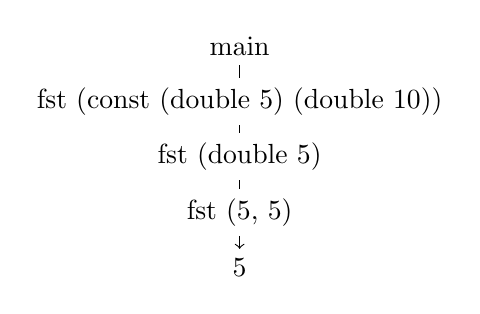
\begin{tikzpicture}[->,node distance=2em]
		\node              (r0) {\fuspel{main}};
		\node[below of=r0] (r1) {\fuspel{fst (const (double 5) (double 10))}};
		\node[below of=r1] (r2) {\fuspel{fst (double 5)}};
		\node[below of=r2] (r3) {\fuspel{fst (5, 5)}};
		\node[below of=r3] (r4) {\fuspel{5}};
		\path[draw] (r0) -- (r1) -- (r2) -- (r3) -- (r4);
	\end{tikzpicture}
	\caption{Basic rewriting example.\label{fig:rewrite:examples:basic}}
\end{figure}

\subsection{The code keyword}
\label{sec:examples:code}

With the \fuspel{code} keyword it is possible to link to C code. This works as
follows:

\begin{lstlisting}
	mul a b = code mul a b;
	sub a b = code sub a b;
	fac 1   = 1;
	fac n   = mul n (fac (sub 1 n));
	main    = fac 3;
\end{lstlisting}

To rewrite a \fuspel{code} expression, all its arguments have to be evaluated
completely. The corresponding C function is looked up and executed on its
arguments. The expression is rewritten with the result of the function call.

The code name \fuspel{mul} stands for integer multiplication, \fuspel{sub} for
subtraction. Hence, the example is rewritten as:

\begin{lstlisting}
	main
	     fac 3
	     mul 3 (     fac (     sub 1 3)        )
	     mul 3 (     fac (code sub 1 3)        )
	     mul 3 (     fac 2                     )
	     mul 3 (     mul 2 (fac (     sub 1 2)))
	     mul 3 (     mul 2 (fac (code sub 1 2)))
	     mul 3 (     mul 2 (fac 1)             )
	     mul 3 (     mul 2 1                   )
	     mul 3 (code mul 2 1                   )
	     mul 3 2
	code mul 3 2
	6
\end{lstlisting}

A complete overview of the \fuspel{code} names can be found in
\autoref{sec:code}.
